\documentclass[a4paper,pagesize 10pt]{scrartcl}

\usepackage{graphicx}
\usepackage{scalefnt}
\usepackage{textfit}
\usepackage{enumitem}
\usepackage{boldline}

\setlist[enumerate]{itemsep=0mm}
\setlist[itemize]{itemsep=0mm}
\begin{document}


\begin{center}{\Huge\textbf{Project Report}}\end{center}
\begin{center}{\Large\textbf{''Analysis of Iterative Closest Point''}}\end{center}
\begin{center}{\small\textbf{Sumit Dugar and Neha Das}}\end{center}


\section*{Abstract}

\textit{Iterative closest Point (ICP) is an algorithm employed to minimize the difference between two point clouds given an initial estimate of the relative pose. It is often used to reconstruct 2D or 3D surfaces from different scans, to localize robots and achieve optimal path planning and to register medical scans. ICP has several steps and each step may be implemented in various ways which give rise to a multitude of ICP variants. In our project, we implement and analyze several variants of ICP, comparing them on the basis of execution speed and quality of the result.}

\section*{Iterative Closest Point Algorithm}
As indicated above, the algorithm for applying iterative closest point to register a source mesh to a target mesh has several steps. We describe these steps in brief below:
\begin{enumerate}
    \item \textbf{Selection:} A set of points are selected from the source mesh. In the vanila implementation, these points are often selected randomly. Selecting more points than less usually leads to a more accurate registration but at the cost of execution speed. 
    \item \textbf{Matching:} Selected points from the source mesh are transformed via the initial estimated relative pose and matched to the points in the target mesh. The aim here is to pair up points in the two meshes that actually both project to the same point in the real world model.
    \item \textbf{Weighing:} The matched points are accordingly weighted. A higher weight is often assigned to a more undesirable pair of matched points. In our implemented variants, we have uniformly weighed all the matched pairs.
    \item \textbf{Rejection:} Of the matched points, we reject the outliers - for instance, we may discard the pairs that are separated by a distance greater than some threshold.
    \item \textbf{Error metric:} We select an error metric for evaluating the matched pairs. For example, a point to point distance metric, or a point to plane distance metric.
    \item \textbf{Optimizing technique:} We must also select an optimization technique for minimizing the error metric for the corresponding pairs from the source and target meshes. For instance, we may opt for linear least squares or non-linear least squares 
\end{enumerate} 

\section*{Implemented Variants}
We will analyze three implementations of ICP that result from a different methodology being used in the steps 1, 2 and 6 of the algorithm as outlined in the above section. We will analyze the advantages and disadvantages of these variants with respect to the convergence speed and output quality. Finally, we will combine the most efficient of these variants and analyze the results from its execution. But first, we shall describe the base implementation that we will be comparing them to.

\subsection*{Baseline}
The baseline ICP we use has the following features:
\begin{itemize}
    \item A fixed number of points are randomly selected from the source mesh.
    \item An attempt is made to match all of the selected points to points in the target mesh by means of a kdd tree and Nearest Neighbor approach
    \item Matched pairs are rejected if the distance between them is greater than a fixed threshold
    \item The error metric to be minimized is selected to be the sum of the point to plane distance between all the matched pairs
    \item A Non-linear least squares optimization technique, specifically Levenberg-Marquardt \cite{L} and \cite{M}, is used to minimize the error. We run the optimization for 10 iterations for the RGBD-Dataset.
\end{itemize}

\subsection*{Multi-resolution ICP}
We introduce a different methodology for step 1 in this scheme. Instead of selecting a fixed number of source points for matching, we change the number of points to be matched as we iterate, effectively moving from matching a coarse resolution of the source mesh to matching a fine resolution of the source mesh (more number of points) as we iterate and refine our solution. Our implementation follows the multiresolution scheme outlined in \cite{H}. \\\\
We sample about one eight of the total source pixels - this is our richest resolution. We resample these points twice to give us our 2nd and third resolutions (see Fig 1). We match the points first in the coarsest resolution and then, as we move through our fixed number of iterations, we increase the resolution. \\\\
\begin{center}
    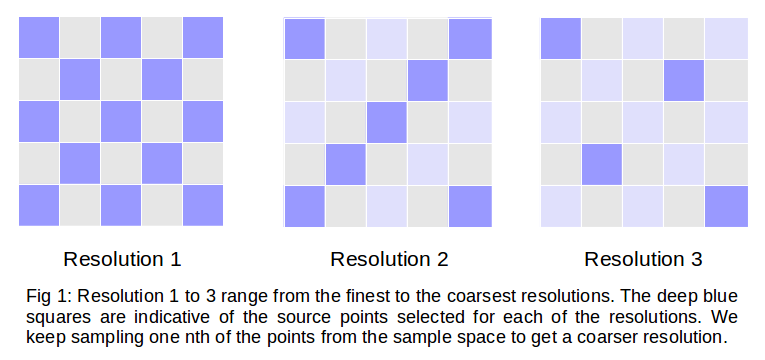
\includegraphics[scale=0.5]{MultiRes.png}
\end{center}
Lessening the number of points in the first few steps results in less accurate registration, but as the resolution is increased in the subsequent iterations, the result improves as well. Additionally, we still have the benefit of a faster convergence speed over the vanilla implementation (see Results).

\subsection*{Projective ICP}
In our baseline implementation of ICP, we use Nearest-Neighbors for calculating matches (Step 2 from Iterative Closest Point Algorithm). Here, we use a much faster method based on the paper by Blais and Levine \cite{blaise}. \\\\
Instead of searching for a neighbor in the whole space of sampled points from the target, we leverage the structure of our 2D image projection of the 3D scene to automatically calculate the closest point in the target sample space (or a tighter search neighborhood for our source point) (see Fig 2). \\\\
\begin{center}
    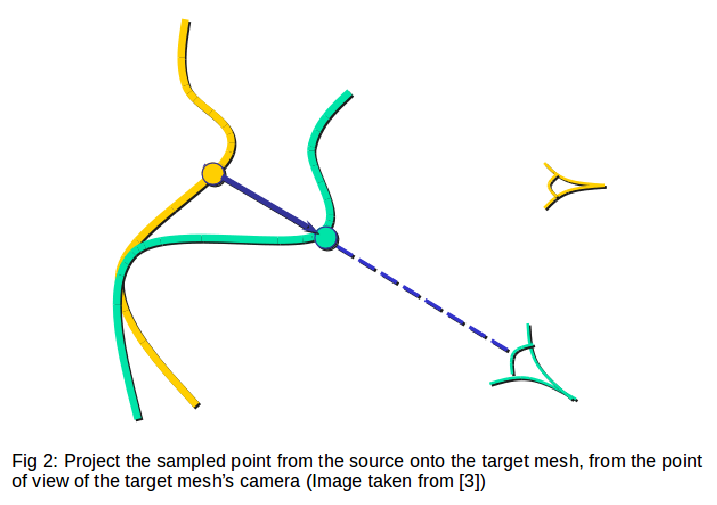
\includegraphics[scale=0.5]{ProjectiveICP.png}
\end{center}
We describe the algorithm for matching in projective ICP below:
\begin{itemize}
    \item Transform a sampled source point by its estimated relative transformation. The initial value for this is often taken to be identity
    \item Project this transformed point on to the target image plane, thus obtaining the row (r) and column (c) of the pixel it maps to.
    \item Project the pixel at (r,c) in the target image back to the 3D camera space.
    \item Calculate the point to plain distance between the transformed point and the matched target point
    \item Discard the match if the distance is beyond the fixed threshold. If not, add to the error metric.
\end{itemize}

This scheme may result in a faster convergence rate as we decrease the neighborhood search area. The search window size dictates the accuracy of the solution and the speed of the algorithm. Increasing the size of the search window results in a higher accuracy but the speed of execution decreases.

\subsection*{Linearized ICP}
In this variant, we replace the baseline's optimization algorithm (Step 6 from Iterative Closest Point Algorithm) - Levenberg-Marquardt (LM) with Singular Value Decomposition (SVD). \\\\
LM is an iterative technique for optimization of a non-linear least squares problem - a generalization of linear least squares. SVD, on the other hand is a stable technique for solving a system of linear equations in one shot.\\\\
So, while LM can can be used to optimize more generalized error functions that may be changing with each iteration (as in ICP), SVD is much quicker, not just because it may converge in one iteration (we also used it for the same number of iterations as the baseline), but also because it takes less compute time than LM which has to calculate Jacobians at each iteration.

\section*{Data}
We perform our analysis on two datasets:

\subsection*{1. Bunny Meshes}
We use the bunny meshes from the exercise \cite{Ex} to demonstrate the effects of the different variants of Iterative Closest Point. Initially, the source (green) and the target (red) meshes are aligned as below:
\begin{center}
    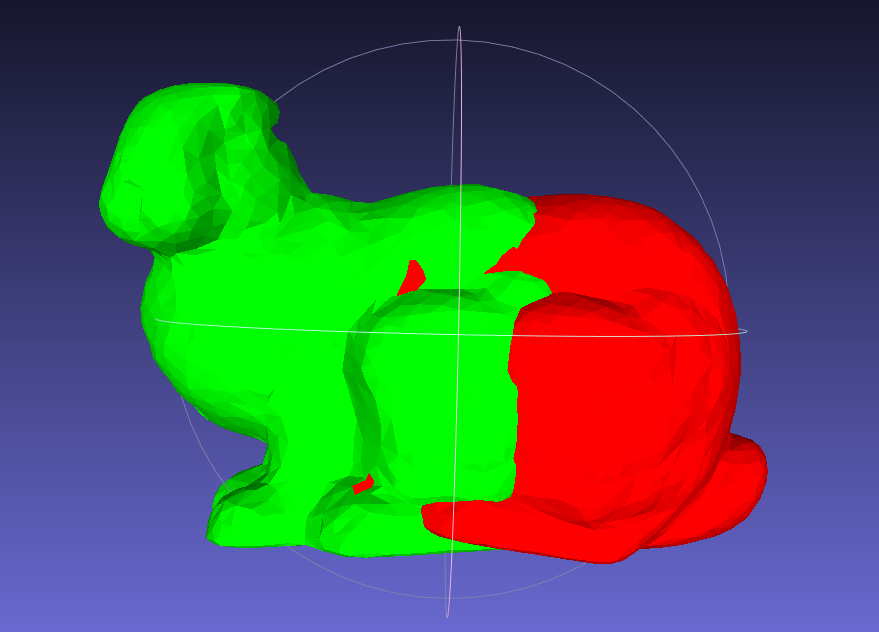
\includegraphics[scale=0.20]{ICP_analysis_bunny_data.png}
\end{center}

\subsection*{2. RGBD Freiburg - xyz}
This data was taken from a public dataset from the Computer Vision Group, TUM. \cite{Frei}. For this sequence, the Kinect was pointed at a typical desk in an office environment. This sequence contains only translatory motions along the principal axes of the Kinect, while the orientation was kept (mostly) fixed. Initially, the source and the target meshes are aligned as below:
\begin{center}
    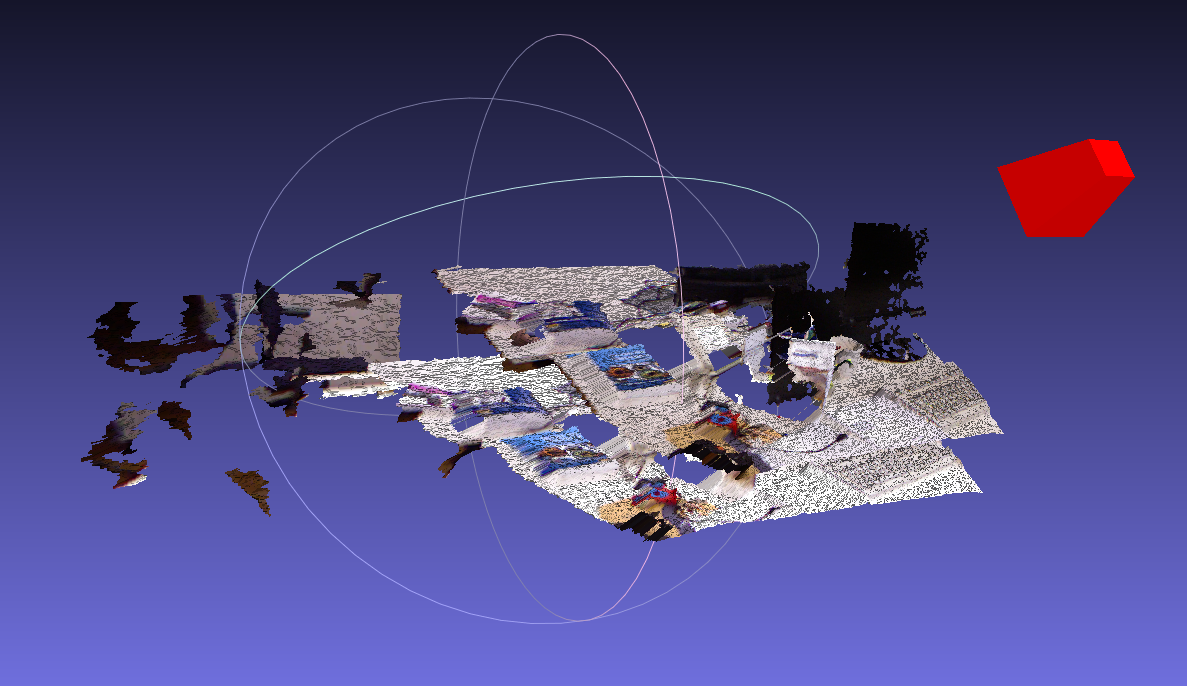
\includegraphics[scale=0.16]{ICP_analysis_room_data.png}
\end{center}

\section*{Results}
A summary of our experimental obsevations are given below:\\\\
\begin{tabular}{| l l | l | l |} 
  \hlineB{2}
   & \textbf{Combinations of Steps 1,2,6} & \textbf{Completion Time} & \textbf{Output Quality}\\ [0.5ex] 
  \hline
  1. & Random Sampling, NN$^1$ and LM$^2$    & Dataset 1: 0.120355 $s$ & Registration Quality is \\
     &                               & Dataset 2: 196.876 $s$ & good in both Datasets$^6$\\ 
  \hline
  2. & Multi-Resolution, NN$^1$ and LM$^2$   & Dataset 1: 0.098971 $s$ & Registration Quality is \\
     &                               & Dataset 2: 105.661 $s$ & good in both Datasets$^6$\\
  \hline
  3. & Random Sampling, Projective       & Dataset 1: N/A          & Registration Quality is \\
     & (Neighborhood of 5 px) and LM$^2$   & Dataset 2: 133.704 $s$ & good in both Datasets$^6$\\
  \hline
  4. & Random Sampling, NN$^1$ and SVD$^3$   & Dataset 1: 0.040289 $s$ & Fails$^4$ in Dataset 1 \\
     & (1 iteration)                     & Dataset 2: 27.1635 $s$ & Good$^5$ for Dataset 2\\
  \hline
  5. & Random Sampling, NN$^1$ and SVD$^3$   & Dataset 1: 0.061886 $s$ & Registration Quality is \\
     &                               & Dataset 2: 85.9964 $s$ & good in both Datasets$^6$\\
  \hline
  6. & Multi-Resolution, Projective      & Dataset 1: N/A          & Registration Quality is \\
     & (Neighborhood of 5 px) and SVD$^3$  & Dataset 2: 29.106 $s$ & good in both Datasets$^6$\\[0.5ex] 
  \hlineB{2}
\end{tabular}
\\\\\\
\tiny{$^1$ Nearest Neighbor Search\\
$^2$ Levenberg-Marquardt\\
$^3$ Singular Value Decomposition\\
$^4$ and $^5$ While SVD (1 iteration) works well with the Freiburg dataset, it fails to completely align the bunny meshes(see Fig 3). This could be because while in the Freiburg dataset, the input meshes were very close (or rather the initial relative pose was nearly accurate), but the bunny meshes were quite some distance apart. Repeated iterations of SVD seemed to align both meshes quite well, however.\\
$^6$ All the outputs are more or less comparable}

\\\\
\begin{center}
    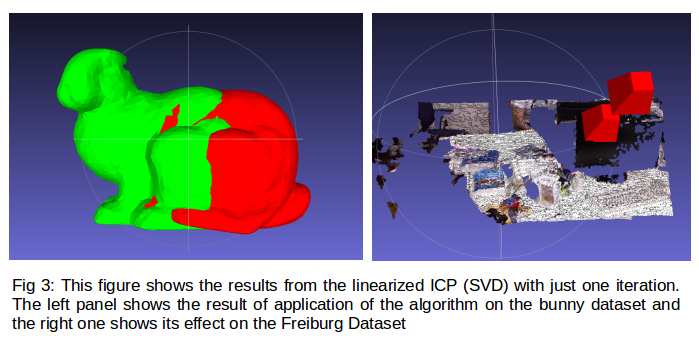
\includegraphics[scale=0.60]{SVD_1_iter.png}
\end{center}
\\\\
\normalsize{The following figures show the output for the rest of the cases in the table. As shown, the quality of the output is more or less the same in these cases:} \\\\
\begin{center}
    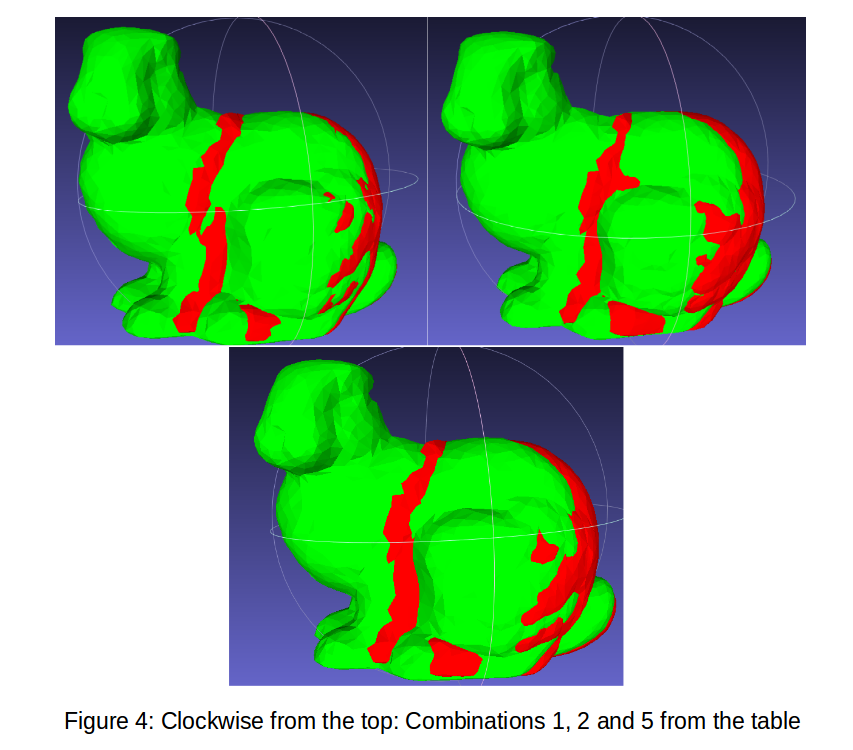
\includegraphics[scale=0.45]{bunny_results.png}
\end{center}

% references
\bibliographystyle{plain}
\bibliography{project_proposal}
\begin{thebibliography}{5}
    \bibitem{H}T. Jost and H. Hugli, "A multi-resolution ICP with heuristic closest point search for fast and robust 3D registration of range images," \textit{Fourth International Conference on 3-D Digital Imaging and Modeling, 2003. 3DIM 2003. Proceedings}
    \bibitem{blaise}Blais, G. and Levine, M, "Registering Multiview Range Data to Create 3D Computer Objects", \textit{Trans. PAMI, Vol. 17, No. 8, 1995}
    \bibitem{PPT}Presentation by Ronen Gvili, "Iterative Closest Point", \textit{www.cs.tau.ac.il/~dcor/Graphics/adv-slides/ICP.ppt}
    \bibitem{L}Levenberg, K, "A Method for the Solution of Certain Problems in Least Squares", \textit{Quart. Appl. Math. 2, 164-168, 1944}
    \bibitem{M}Marquardt, D, "An Algorithm for Least-Squares Estimation of Nonlinear Parameters." \textit{SIAM J. Appl. Math. 11, 431-441, 1963}
    \bibitem{Ex}Exercise 3. from the lecture "3D Scanning and Analysis", \textit{Technical University of Munich}
    \bibitem{Frei}J. Sturm etal., "A Benchmark for the Evaluation of RGB-D SLAM Systems", \textit{Proc. of the International Conference on Intelligent Robot Systems (IROS) 2012 Oct.}
\end{thebibliography}


\end{document}